\documentclass[border=2pt]{standalone}
\usepackage{circuitikz}
\begin{document}
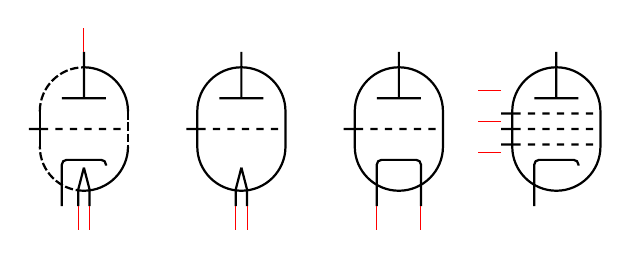
\begin{tikzpicture}
  \node[triode,filament,circuitikz/tubes/partial borders=121212,
    circuitikz/tubes/partial border dash={{3pt}{1pt}}] (F) at (0,0) {};
  \node[triode,nocathode,filament] (N) at (2,0) {};
  \node[triode,fullcathode] (C) at (4,0) {};
  \node[pentode] (P) at (6,0) {};
  \draw[red] (F.anode) -- ++(0,.3)
    (F.filament 1) -- ++(0,-.3) (F.filament 2) -- ++(0,-.3)
    (N.filament 1) -- ++(0,-.3) (N.filament 2) -- ++(0,-.3)
    (C.cathode 1) -- ++(0,-.3) (C.cathode 2) -- ++(0,-.3);
  \ctikzset{tubes/grid shift=.1,tubes/grid separation=.4}
  \draw[red] (P.control) -- ++(-.3,0) (P.screen) -- ++(-.3,0)
    (P.suppressor) -- ++(-.3,0);
\end{tikzpicture}
\end{document}
